\chapter{Formal Mathematical Statements}
\begin{outcome}
\begin{itemize}
\item Establish needed mathematical notation
\item Understand structural results pertaining to linear programs
\item Develop an intuition for why these results are true
\end{itemize}
\end{outcome}
In this chapter, we formalize some of the mathematics about linear programs.  We define some notation here and then state and prove several theorems.   

\begin{warn}
In this section, we provide rigirous mathematical proofs of several results.  For this course, you do not need to be able to reproduce these proofs.  However, try to understand the concepts and have a visual image in your head of why these results are true.
\end{warn}
\subsection{Vectors and Their Properties}

\textbf{Vectors:}  
A vector is a mathematical object that represents a point in space or a direction. In \(n\)-dimensional real space (\(\mathbb{R}^n\)), a vector \(\mathbf{v}\) is written as an ordered list of \(n\) elements:  
\[
\mathbf{v} = (v_1, v_2, \dots, v_n).
\]  
Vectors can be written in two forms: as a row vector \([v_1, v_2, \dots, v_n]\) or as a column vector:
\[
\mathbf{v} = \begin{bmatrix} v_1 \\ v_2 \\ \vdots \\ v_n \end{bmatrix}.
\]  
In linear programming, vectors are used to represent variables, constraints, and directions in optimization problems.

\medskip  
\textbf{Vector Operations:}  
Vector operations form the building blocks for linear programming, enabling the manipulation of decision variables and constraints.

\begin{description}
    \item[Addition:]  
    Vectors of the same dimension can be added componentwise. For example, if \(\mathbf{v} = (2, 3)\) and \(\mathbf{u} = (3, 2)\), their sum is:  
    \[
    \mathbf{v} + \mathbf{u} = (2+3, 3+2) = (5, 5).
    \]  
    This operation is essential in modeling systems where contributions of multiple variables are combined.

    \item[Scalar Multiplication:]  
    A vector can be scaled by multiplying it with a scalar (constant). For example, if \(k = 2\) and \(\mathbf{v} = (2, 3)\), then:
    \[
    k\mathbf{v} = (2 \cdot 2, 3 \cdot 2) = (4, 6).
    \]  
    Scalar multiplication adjusts the magnitude of a vector while retaining its direction, a key concept in scaling constraints or objectives in linear programming.

    \item[Inner (Dot) Product:]  
    The dot product of two vectors \(\mathbf{v}\) and \(\mathbf{u}\) of the same size is calculated as:
    \[
    \mathbf{v} \cdot \mathbf{u} = \sum_{i=1}^n v_i u_i.
    \]  
    For example, if \(\mathbf{v} = (2, 3)\) and \(\mathbf{u} = (3, 2)\), then:
    \[
    \mathbf{v} \cdot \mathbf{u} = 2 \cdot 3 + 3 \cdot 2 = 10.
    \]  
    The dot product is crucial in defining constraints and objective functions in linear programming, as it represents weighted sums of variables.
\end{description}

\subsection{Linear Combinations and Related Concepts}

\textbf{Linear Combination:}  
A vector \(\mathbf{u}\) is a linear combination of vectors \(\mathbf{v}^1, \mathbf{v}^2, \dots, \mathbf{v}^k\) if:
\[
\mathbf{u} = \sum_{i=1}^k \lambda_i \mathbf{v}^i,
\]
where \(\lambda_1, \lambda_2, \dots, \lambda_k\) are scalars. If all scalars are non-negative (\(\lambda_i \geq 0\)), the combination is called a \emph{non-negative linear combination}. Linear combinations are used in linear programming to express feasible solutions as sums of variable contributions.

\medskip  
\textbf{Convex Combination:}  
A vector \(\mathbf{u}\) is a convex combination of vectors \(\mathbf{v}^1, \mathbf{v}^2, \dots, \mathbf{v}^k\) if:
\[
\mathbf{u} = \sum_{i=1}^k \lambda_i \mathbf{v}^i, \quad \text{where } \lambda_i \geq 0 \text{ and } \sum_{i=1}^k \lambda_i = 1.
\]
Convex combinations are fundamental to linear programming because they describe feasible regions (e.g., convex polyhedra).

\begin{definition}{Linear Independence}{}{}
A set of vectors \( \{ \mathbf{v}^1, \mathbf{v}^2, \dots, \mathbf{v}^k \} \subseteq \mathbb{R}^n \) is said to be \emph{linearly independent} if the only solution to the equation
\[
\lambda_1 \mathbf{v}^1 + \lambda_2 \mathbf{v}^2 + \dots + \lambda_k \mathbf{v}^k = \mathbf{0}
\]
is \( \lambda_1 = \lambda_2 = \dots = \lambda_k = 0 \).  

Equivalently, no vector in the set can be written as a linear combination of the others.
\end{definition}

\textbf{Examples:}
\begin{itemize}
    \item The vectors \( \begin{bmatrix}1\\0\end{bmatrix} \) and \( \begin{bmatrix}0\\1\end{bmatrix} \) in \( \mathbb{R}^2 \) are linearly independent.
    \item The vectors \( \begin{bmatrix}1\\2\end{bmatrix} \) and \( \begin{bmatrix}2\\4\end{bmatrix} \) are linearly dependent, since the second is a scalar multiple of the first.
\end{itemize}

\vspace{1em}

\begin{definition}{Linear Independence of Rows or Columns}{}{}
Let \( A \in \mathbb{R}^{m \times n} \) be a matrix.

\begin{itemize}
  \item The rows of \( A \) are said to be \emph{linearly independent} if no row can be written as a linear combination of the other rows.
  
  \item The columns of \( A \) are \emph{linearly independent} if no column can be written as a linear combination of the other columns.
  
  \item In either case, the vectors are linearly independent if the only solution to the homogeneous system \( A \mathbf{x} = \mathbf{0} \) (or \( A^\top \mathbf{y} = \mathbf{0} \)) is the trivial solution \( \mathbf{x} = \mathbf{0} \) (or \( \mathbf{y} = \mathbf{0} \)).
\end{itemize}
\end{definition}

\textbf{Examples:}
\begin{itemize}
    \item The matrix \( A = \begin{bmatrix}1 & 0 \\ 0 & 1\end{bmatrix} \) has both linearly independent rows and columns.
    \item The matrix \( A = \begin{bmatrix}1 & 2 \\ 2 & 4\end{bmatrix} \) has linearly dependent rows and columns; the second row is twice the first, and the second column is twice the first.
\end{itemize}

\vspace{1em}

\begin{definition}{Rank of a Matrix}{}{}
Let \( A \in \mathbb{R}^{m \times n} \). The \emph{rank} of \( A \), denoted \( \operatorname{rank}(A) \), is the maximum number of linearly independent rows or columns of \( A \).

Equivalently, \( \operatorname{rank}(A) \) is:
\begin{itemize}
  \item the dimension of the row space of \( A \),
  \item the dimension of the column space of \( A \),
  \item the number of pivot columns in the reduced row echelon form of \( A \),
  \item the largest integer \( r \) such that \( A \) has an \( r \times r \) submatrix with nonzero determinant.
\end{itemize}
\end{definition}

\textbf{Examples:}
\begin{itemize}
    \item The matrix \( A = \begin{bmatrix}1 & 2 \\ 3 & 4\end{bmatrix} \) has full rank 2.
    \item The matrix \( A = \begin{bmatrix}1 & 2 \\ 2 & 4\end{bmatrix} \) has rank 1, since the second row is a multiple of the first.
\end{itemize}

\vspace{1em}

\begin{definition}{Linearly Independent Constraints}{}{}
Let \( A \mathbf{x} \leq \mathbf{b} \) be a system of linear inequalities, where each constraint corresponds to a row \( A_i \mathbf{x} \leq b_i \). A subset of these constraints is said to be \emph{linearly independent} at a point \( \mathbf{x} \in \mathbb{R}^n \) if the set of row vectors \( \{ A_i : A_i \mathbf{x} = b_i \} \) (i.e., the tight constraints at \( \mathbf{x} \)) is linearly independent.

Equivalently, the tight constraints at \( \mathbf{x} \) are linearly independent if the matrix \( A_I \) formed by stacking the tight rows satisfies
\[
\operatorname{rank}(A_I) = |I|,
\]
where \( I := \{ i : A_i \mathbf{x} = b_i \} \).
\end{definition}

\textbf{Examples:}
\begin{itemize}
    \item Let \( A \mathbf{x} \leq \mathbf{b} \) be the system:
    \[
    \begin{aligned}
    x_1 &\leq 1 \\
    x_2 &\leq 1 \\
    x_1 + x_2 &\leq 2
    \end{aligned}
    \]
    At \( \mathbf{x} = (1, 1) \), all three constraints are tight. The first two have row vectors \( [1,0] \) and \( [0,1] \), which are linearly independent. The third is \( [1,1] \), which is a linear combination of the first two. So only two of the tight constraints are linearly independent.
    
    \item In contrast, for the system:
    \[
    \begin{aligned}
    x_1 &\leq 0 \\
    x_2 &\leq 0
    \end{aligned}
    \]
    the point \( \mathbf{x} = (0,0) \) has both constraints tight, and their rows \( [1,0] \), \( [0,1] \) are linearly independent. Hence the tight constraints are linearly independent at that point.
\end{itemize}


\section{Algebraic Proof - Exists Optimial Solution at a Vertex}



\begin{definition}{Vertex}{}{}
Let \( P = \{ \mathbf{x} \in \mathbb{R}^n : A \mathbf{x} \leq \mathbf{b} \} \) be a polyhedron.  
A point \( \mathbf{x} \in P \) is called a \emph{vertex} (or \emph{corner point}) of \( P \) if it is the unique solution to a system of \( n \) linearly independent constraints that are tight at \( \mathbf{x} \).  
In other words, \( \mathbf{x} \) is a vertex if there exists a subset \( I \subseteq \{1, \dots, m\} \) such that:
\begin{itemize}
  \item \( A_i \mathbf{x} = b_i \) for all \( i \in I \),
  \item The rows \( \{ A_i : i \in I \} \) are linearly independent,
  \item \( |I| = n \).
\end{itemize}
\end{definition}

\begin{theorem}{}{}{}
Let \( \max \{ \mathbf{c}^\top \mathbf{x} : A \mathbf{x} \leq \mathbf{b} \} \) be a linear program with a nonempty, bounded feasible region \( P \).  
If an optimal solution exists, then there exists an optimal solution that is a vertex of \( P \).
\end{theorem}

\begin{proof}
Let \( \mathbf{x}^* \in P \) be an optimal solution, and suppose for contradiction that \( \mathbf{x}^* \) is \emph{not} a vertex.

Define the index set of tight (active) constraints at \( \mathbf{x}^* \) as
\[
I := \{ i \in \{1, \dots, m\} : A_i \mathbf{x}^* = b_i \},
\]
where \( A_i \) is the $i$th row of \( A \). Let \( A_I \) be the submatrix of \( A \) consisting of the rows indexed by \( I \).

Since \( \mathbf{x}^* \) is not a vertex, the tight constraints are linearly dependent: \( \operatorname{rank}(A_I) < n \). Therefore, the homogeneous system \( A_I \mathbf{d} = 0 \) has a nonzero solution \( \mathbf{d} \in \mathbb{R}^n \setminus \{0\} \).

Consider the line \( \mathbf{x}(t) := \mathbf{x}^* + t \mathbf{d} \) for small \( t \in \mathbb{R} \). For all \( i \in I \), we have:
\[
A_i \mathbf{x}(t) = A_i \mathbf{x}^* + t A_i \mathbf{d} = b_i + 0 = b_i,
\]
so the tight constraints remain tight along the line.

For any \( i \notin I \), we have \( A_i \mathbf{x}^* < b_i \). Since \( A_i \mathbf{d} \) is bounded, we can choose a small enough \( \varepsilon > 0 \) such that for all \( t \in [-\varepsilon, \varepsilon] \), the inequality \( A_i \mathbf{x}(t) \leq b_i \) holds. Thus, for small \( t \), \( \mathbf{x}(t) \in P \).

Now define the objective value along this line: 
\[
z(t) := \mathbf{c}^\top \mathbf{x}(t) = \mathbf{c}^\top \mathbf{x}^* + t \cdot (\mathbf{c}^\top \mathbf{d}).
\]

\begin{itemize}
\item If \( \mathbf{c}^\top \mathbf{d} > 0 \), then for small \( t > 0 \), \( \mathbf{x}(t) \in P \) and \( \mathbf{c}^\top \mathbf{x}(t) > \mathbf{c}^\top \mathbf{x}^* \), contradicting optimality of \( \mathbf{x}^* \).
\item If \( \mathbf{c}^\top \mathbf{d} < 0 \), then for small \( t < 0 \), same contradiction.
\item If \( \mathbf{c}^\top \mathbf{d} = 0 \), then \( \mathbf{x}(t) \) is also optimal for all small \( t \), and we can move in both directions while maintaining feasibility and optimality.
\end{itemize}

In all cases, we can find another feasible optimal point along the line \( \mathbf{x}(t) \), with the same or better objective value. Moreover, we can choose such a point with a strictly larger set of linearly independent tight constraints. Repeating this process, we eventually reach an optimal point at which the tight constraints form a full-rank system (rank \( n \)), which uniquely determines the point. Such a point is, by definition, a vertex.

This contradicts our assumption that no optimal vertex exists.
\end{proof}


\section{Convexity}
A key property that will enable efficient algorithms is \emph{convexity}.  This comes in the form of \emph{convex sets} and \emph{convex functions}.  Then the constraints to an optimization problem form a  convex set and the objective function is a convex function, then we say that it is a convex optimization problem.

We explain these definitions in the next two subsections.
\subsection{Convex Sets}

\begin{definition}{Convex Combination}{}
Given two points $\x,\y$, a \emph{convex combination} is any point $z$ that lies on the line between $\x$ and $\y$.  Algebraically, a \emph{convex combination} is any point $\z$ that can be represented as $\z = \lambda \x + (	1-\lambda) \y $ for some multiplier $\lambda \in [0,1]$.
\end{definition}

\begin{figure}[h]
\begin{center}
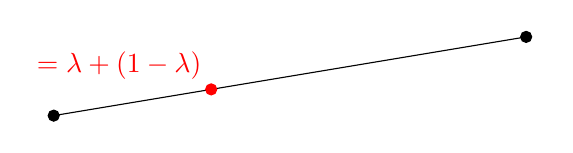
\begin{tikzpicture}

% Define the points
\coordinate (x) at (0,0);
\coordinate (y) at (6,1);
\coordinate (z) at (2/3*0 + 1/3*6, 2/3*0 + 1/3*1);

% Plot the line segment between x and y
\draw (x) -- (y);

% Mark the points with dots and labels
\filldraw [black] (x) circle (2pt) node[anchor=east] {$\x$};
\filldraw [black] (y) circle (2pt) node[anchor=west] {$\y$};
\filldraw [red] (z) circle (2pt) node[anchor=south east] {$\z = \lambda \x + (1-\lambda)\y$};

\end{tikzpicture}
\end{center}
\caption{A convex combination of the points $\x$ and $\y$ is given by $\z = \lambda \x + (1-\lambda)\y$ with any $\lambda \in [0,1]$.  Here we demonstrate this using $\lambda = 2/3$.  }
\end{figure}



\begin{definition}{Convex Set}{}
A set $C$ is convex if it contains all convex combinations of points in $C$.  That is, for any $\x,\y \in C$, it holds that $ \lambda \x + (1-\lambda) \y \in C$ for all $\lambda \in [0,1]$.
\end{definition}


\begin{figure}[h]
  \begin{subfigure}[b]{0.45\textwidth}
    \centering
    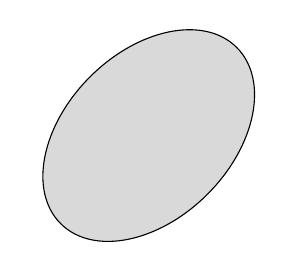
\begin{tikzpicture}
        \draw[rotate=-45,fill=gray!30, thin] (0,0) ellipse (30pt and 45pt);
    \end{tikzpicture}
    \caption{Convex Set}
    \label{a}
  \end{subfigure}
  \begin{subfigure}[b]{0.45\textwidth}
    \centering
    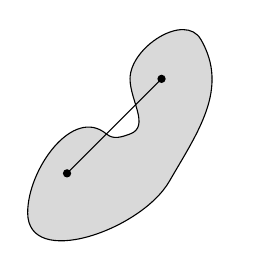
\begin{tikzpicture}
        \useasboundingbox (-1,-1.35) rectangle (1.5,1.35); 
        \draw[fill=gray!30, thin] (0,0) to [out=140,in=90] (-1,-1)
        to [out=-90,in=240] (0.8,-0.6)
        to [out=60,in=-60] (1.2,1.2)
        to [out=120,in=90] (0.3,0.7)
        to [out=-90,in=20] (0.3,0)
        to [out=200,in=-40] (0,0);
        \draw[thin] (-0.5,-0.5) -- (0.7,0.7);
        \fill (-0.5,-0.5) circle[radius=1.5pt];
        \fill (0.7,0.7) circle[radius=1.5pt];
    \end{tikzpicture}
    \caption{Non-convex Set}
    \label{b}
  \end{subfigure}
\end{figure}




%\begin{definition}{Convex Sets}{}
%A set $S$ is \emph{convex} if for any two points in $S$, the entire line segment between them is also contained in $S$.
%That is, for any $x,y \in S$
%$$
%\lambda x + (1-\lambda y) \in S \ \ \text{ for all } \lambda \in [0,1].
%$$
%\end{definition}


    


Some examples of convex sets are:
\begin{enumerate}
    \item \emph{Hyperplane}  $H = \{\x \in \R^n : \a^\top \x = b\}$
    \item \emph{Halfspace}   $H = \{ \x \in \R^n : \a^\top \x \leq b\}$
    \item \emph{Polyhedron}  $P = \{\x \in \R^n : A\x \leq \b\}$
    \item \emph{Ball} $B = \{ \x \in \R^n : \sum_{i=1}^n x_i^2 \leq 1\}$
    %\item \emph{Second Order Cone} $S = \{ (\x,t) \in \R^n \times \R : \sum_{i=1}^n x_i^2 \leq t^2 \}$
\end{enumerate}


\begin{figure}[h!]
\centering
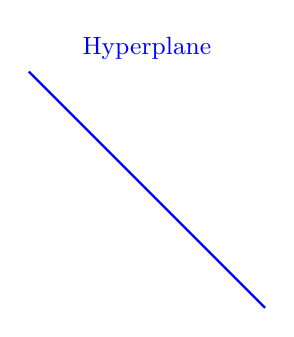
\begin{tikzpicture}[scale=1]
    % Hyperplane
    \draw[blue, thick] (-1.5,1.5) -- (1.5,-1.5);
    \node[blue] at (0,1.8) {\small Hyperplane};
    % Axes
   % \draw[->,thick] (-2,0) -- (2,0) node[right] {$x_1$};
    %\draw[->,thick] (0,-2) -- (0,2) node[above] {$x_2$};
\end{tikzpicture}
\hfill
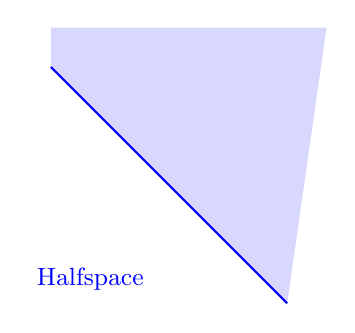
\begin{tikzpicture}[scale=1]
    % Halfspace
    \fill[blue!30,opacity=0.5] (-1.5,1.5) -- (1.5,-1.5) -- (2,2) -- (-1.5,2) -- cycle;
    \draw[blue, thick] (-1.5,1.5) -- (1.5,-1.5);
    \node[blue] at (-1,-1.2) {\small Halfspace};
    % Axes
    %\draw[->,thick] (-2,0) -- (2,0) node[right] {$x_1$};
    %\draw[->,thick] (0,-2) -- (0,2) node[above] {$x_2$};
\end{tikzpicture}
\hfill
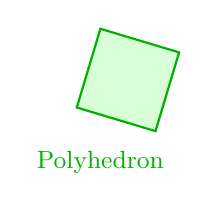
\begin{tikzpicture}[scale=1]
    % Polyhedron
    \fill[green!30,opacity=0.5] (0.5,0.5) -- (1.5,0.2) -- (1.2,-0.8) -- (0.2,-0.5) -- cycle;
    \draw[green!70!black, thick] (0.5,0.5) -- (1.5,0.2) -- (1.2,-0.8) -- (0.2,-0.5) -- cycle;
    \node[green!70!black] at (0.5,-1.2) {\small Polyhedron};
    % Axes
    %\draw[->,thick] (-2,0) -- (2,0) node[right] {$x_1$};
    %\draw[->,thick] (0,-2) -- (0,2) node[above] {$x_2$};
\end{tikzpicture}
\hfill
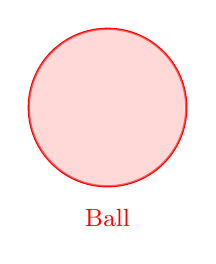
\begin{tikzpicture}[scale=1]
    % Ball
    \draw[red, thick] (0,0) circle (1cm);
    \fill[red!30,opacity=0.5] (0,0) circle (1cm);
    \node[red] at (0,-1.4) {\small Ball};
    % Axes
    %\draw[->,thick] (-2,0) -- (2,0) node[right] {$x_1$};
    %\draw[->,thick] (0,-2) -- (0,2) node[above] {$x_2$};
\end{tikzpicture}
%\hfill
%\begin{tikzpicture}[scale=1.5]
%    % Second Order Cone
%    \draw[orange, thick] (-1,0) -- (0,2) -- (1,0);
%    \fill[orange!30,opacity=0.5] (-1,0) -- (0,2) -- (1,0) -- cycle;
%    \node[orange] at (0,-1.4) {\small Second Order Cone: $\{(\mathbf{x}, t) \in \mathbb{R}^n \times \mathbb{R} : \|\mathbf{x}\|^2 \leq t^2\}$};
%    % Axes
%    \draw[->,thick] (-2,0) -- (2,0) node[right] {$x_1$};
%    \draw[->,thick] (0,-2) -- (0,2) node[above] {$x_2$};
%\end{tikzpicture}

\end{figure}





\begin{example}{Proof that a Polyhedron is Convex}{polyhedron-convex}
Let \( P \) be a polyhedron defined by:
\[ P = \{\mathbf{x} \in \mathbb{R}^n : A\mathbf{x} \leq \mathbf{b}\} \]
where \( A \) is an \( m \times n \) matrix and \( \mathbf{b} \) is an \( m \times 1 \) vector.\\

To prove the convexity of \( P \), we'll use the definition of convexity: For any \( \mathbf{x}, \mathbf{y} \in P \) and any \( \lambda \in [0,1] \), the point \( \mathbf{z} = \lambda \mathbf{x} + (1-\lambda) \mathbf{y} \) must also belong to \( P \).

Let \( \mathbf{x}, \mathbf{y} \in P \). Then, by the definition of \( P \), we have:
\[ A\mathbf{x} \leq \mathbf{b} \ \ \ \text{ and } \ \ \  A\mathbf{y} \leq \mathbf{b} \]

We want to demonstrate the inequality \( A\mathbf{z} \leq \mathbf{b} \). 
We do this in just a few lines:
\begin{align*}
A\mathbf{z} &= A(\lambda \mathbf{x} + (1-\lambda) \mathbf{y}) & \text{Substituting the expression for \( \mathbf{z} \)}\\
&=\lambda A\mathbf{x} + (1-\lambda) A\mathbf{y} & \text{Expanding the matrix-vector product}\\
&\leq \lambda \mathbf{b} + (1-\lambda) \mathbf{b} & \text{Explanation below}\\
& = \mathbf{b}
\end{align*}
The inequality above uses the fact that \( A\mathbf{x} \leq \mathbf{b} \) and \( A\mathbf{y} \leq \mathbf{b} \), and since \( \lambda \) is in the interval \([0,1]\), it follows that:
\[ \lambda A\mathbf{x} \leq \lambda \mathbf{b}  \ \ \ 
\text{ and } \ \ \ 
(1-\lambda) A\mathbf{y} \leq (1-\lambda) \mathbf{b} \]

The computation shows that \( \mathbf{z} = \lambda \mathbf{x} + (1-\lambda) \mathbf{y} \) satisfies \( A\mathbf{z} \leq \mathbf{b} \) and therefore \( \mathbf{z} \in P \).

This shows that the polyhedron \( P \) is convex.
\end{example}




\begin{lemma}{Intersection of Convex Sets is Convex}{}
Let $C_1$ and $C_2$ be convex sets.  Then the intersection $C_1 \cap C_2$ is convex.  
In particular, 
$$C_1 \cap C_2 := \{ \x :  \x \in C_1 \ \text{ and } \x \in C_2\}.
$$
\end{lemma}

\begin{figure}[h]
\begin{center}
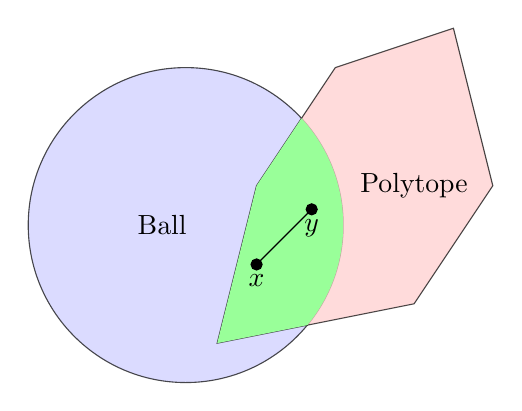
\begin{tikzpicture}

% Draw the circle (ball in 2D) slightly to the left
\filldraw[blue!20, opacity=0.7, draw = black] (0.1,1.5) circle (2cm);

% Draw the 6-vertex polytope slightly to the right
\filldraw[red!20, opacity=0.7, draw = black] (0.5,0) -- (3,0.5) -- (4,2) -- (3.5,4) -- (2,3.5) -- (1,2) -- cycle;

% Shade the intersection
\begin{scope}
  \clip (0.1,1.5) circle (2cm);
  \fill[green!40] (0.5,0) -- (3,0.5) -- (4,2) -- (3.5,4) -- (2,3.5) -- (1,2) -- cycle;
\end{scope}

% Label the circle and polytope
\node at (-0.2,1.5) {Ball};
\node at (3,2) {Polytope};

% Define the points
\coordinate (x) at (1,1);
\coordinate (y) at (1.7,1.7);
\coordinate (z) at (2/3*1 + 1/3*1.7, 2/3*1 + 1/3*1.7);

% Plot the line segment between x and y
\draw (x) -- (y);

% Mark the points with dots and labels
\filldraw [black] (x) circle (2pt) node[anchor=north] {$x$};
\filldraw [black] (y) circle (2pt) node[anchor=north] {$y$};
%\filldraw [red] (z) circle (2pt) node[anchor=south east] {};%$z = \lambda x + (1-\lambda)y$};
\end{tikzpicture}\vspace{1cm}
\end{center}
\caption{The green intersection of the convex sets that are the ball and the polytope is also convex. This can be seen by considering any points $x,y \in \text{Ball} \cap \text{Polytope}$.  Since Ball is convex, the line segment between $x$ and $y$ is completey contained in Ball.  And similarly, the line segment is completely contained in Polytope.  Hence, the line segment is also contained in the intersection.  This is how we can reason that the intersection is also convex.} 
\end{figure}




\medskip  
\textbf{Linear Independence:}  
Vectors \(\mathbf{v}^1, \mathbf{v}^2, \dots, \mathbf{v}^k\) are linearly independent if the only solution to:
\[
\sum_{i=1}^k \lambda_i \mathbf{v}^i = \mathbf{0}
\]
is \(\lambda_1 = \lambda_2 = \cdots = \lambda_k = 0\). In \(\mathbb{R}^2\), two vectors are linearly dependent if they lie on the same line. Linear independence is critical in linear programming to ensure constraints are non-redundant.

\subsection{Spanning Sets and Basis}

\textbf{Spanning Set:}  
A set of vectors \(\mathbf{v}^1, \mathbf{v}^2, \dots, \mathbf{v}^k\) spans \(\mathbb{R}^m\) if any vector in \(\mathbb{R}^m\) can be expressed as a linear combination of these vectors:
\[
\sum_{i=1}^m \lambda_i \mathbf{v}^i.
\]

\textbf{Basis:}  
A set of vectors \(\mathbf{v}^1, \mathbf{v}^2, \dots, \mathbf{v}^m\) is a basis for \(\mathbb{R}^m\) if:
\begin{itemize}
    \item The vectors span \(\mathbb{R}^m\).
    \item The vectors are linearly independent.
\end{itemize}
In linear programming, the concept of a basis is used to identify corner points of the feasible region.

\subsection{Convex and Polyhedral Sets}

\textbf{Convex Set:}  
A set \(C \subseteq \mathbb{R}^n\) is convex if, for any two points \(\mathbf{v}^1, \mathbf{v}^2 \in C\), the line segment joining them lies entirely within \(C\):
\[
\lambda \mathbf{v}^1 + (1 - \lambda) \mathbf{v}^2 \in C, \quad \forall \lambda \in [0, 1].
\]
Convex sets form the feasible regions in linear programming problems.

\textbf{Polyhedral Set:}  
A polyhedral set is the intersection of finitely many half-spaces, described as:
\[
P= \{\mathbf{x} : A \mathbf{x} \leq \mathbf{b}, \, \mathbf{x} \geq \mathbf{0}\}.
\]
Polyhedral sets are convex and represent the feasible regions of linear programming models.

%
%\begin{theorem}{Convexity of Polyhedra}{}
%\label{thm:polyhedra_convex}
%A polyhedron, defined as the intersection of finitely many half-spaces, is a convex set.
%\end{theorem}
%
%\begin{proof}
%Let \( P \) be a polyhedron in \(\mathbb{R}^n\) defined by the intersection of finitely many half-spaces:
%\[
%P = \{\mathbf{x} \in \mathbb{R}^n : A\mathbf{x} \leq \mathbf{b}\},
%\]
%where \(A\) is an \(m \times n\) matrix, \(\mathbf{x} \in \mathbb{R}^n\) is a variable vector, and \(\mathbf{b} \in \mathbb{R}^m\) is a constant vector.
%
%To prove \(P\) is convex, we must show that for any two points \(\mathbf{x}_1, \mathbf{x}_2 \in P\) and any \(\lambda \in [0, 1]\), the point:
%\[
%\mathbf{x}_\lambda = \lambda \mathbf{x}_1 + (1 - \lambda) \mathbf{x}_2
%\]
%also lies in \(P\).
%
%Since \(\mathbf{x}_1, \mathbf{x}_2 \in P\), they satisfy:
%\[
%A\mathbf{x}_1 \leq \mathbf{b} \quad \text{and} \quad A\mathbf{x}_2 \leq \mathbf{b}.
%\]
%By linearity of matrix multiplication and scalar multiplication, for any \(\lambda \in [0, 1]\),
%\[
%A\mathbf{x}_\lambda = A(\lambda \mathbf{x}_1 + (1 - \lambda) \mathbf{x}_2) = \lambda A\mathbf{x}_1 + (1 - \lambda) A\mathbf{x}_2.
%\]
%Using the inequality \(A\mathbf{x}_1 \leq \mathbf{b}\) and \(A\mathbf{x}_2 \leq \mathbf{b}\), we know:
%\[
%\lambda A\mathbf{x}_1 + (1 - \lambda) A\mathbf{x}_2 \leq \lambda \mathbf{b} + (1 - \lambda) \mathbf{b} = \mathbf{b}.
%\]
%Thus, \(\mathbf{x}_\lambda \in P\).
%
%Since \(\mathbf{x}_\lambda\) is in \(P\) for all \(\lambda \in [0, 1]\), it follows that \(P\) is convex.
%\end{proof}
%
%

\textbf{Extreme Points:}  
An extreme point of a polyhedral set \(C\) is a point that cannot be written as a convex combination of other points in \(C\). Linear programming solutions often occur at extreme points, as guaranteed by fundamental theorems of linear programming.

\begin{lemma}{Objective Values on a Line Segment}{}
\label{lemma:objective_bound}
Given two points \(\mathbf{x}, \mathbf{y} \in \mathbb{R}^n\), a linear function evaluated at any point on the line segment between \(\mathbf{x}\) and \(\mathbf{y}\) is bounded above by the maximum of the evaluations at \(\mathbf{x}\) and \(\mathbf{y}\). Formally, for any \(\mathbf{c} \in \mathbb{R}^n\),
\[
\min\{\mathbf{c}^\top \mathbf{x}, \mathbf{c}^\top \mathbf{y}\} \leq \mathbf{c}^\top \mathbf{z} \leq \max\{\mathbf{c}^\top \mathbf{x}, \mathbf{c}^\top \mathbf{y}\}.
\]
where \(\mathbf{z} = \lambda \mathbf{x} + (1-\lambda) \mathbf{y}\) for some $\lambda \in (0,1)$.

Either both of these inequalities are strict, or they are both held at equality.
\end{lemma}

\begin{proof}
Expanding $\mathbf{c}^\top \mathbf{z}$ based on the definition
\begin{align*}
\mathbf{c}^\top \mathbf{z}  &= \mathbf{c}^\top \mathbf{z} (\lambda \mathbf{x} + (1-\lambda) \mathbf{y}) & \text{Replace forumla for $\mathbf{z}$}\\
& =  \mathbf{c}^\top \lambda\mathbf{x} +  \mathbf{c}^\top (1-\lambda)\mathbf{y} & \text{ use distributivity}\\
& = \lambda \mathbf{c}^\top \mathbf{x} + (1-\lambda) \mathbf{c}^\top\mathbf{y} & \text{ use linearity}
\end{align*}


This equation expresses \(\mathbf{c}^\top \mathbf{z}\) as a convex combination of \(\mathbf{c}^\top \mathbf{x}\) and \(\mathbf{c}^\top \mathbf{y}\). Since \(\lambda \in [0, 1]\), we know \(\lambda \geq 0\) and \(1-\lambda \geq 0\), ensuring that the combination is convex.


\begin{center}
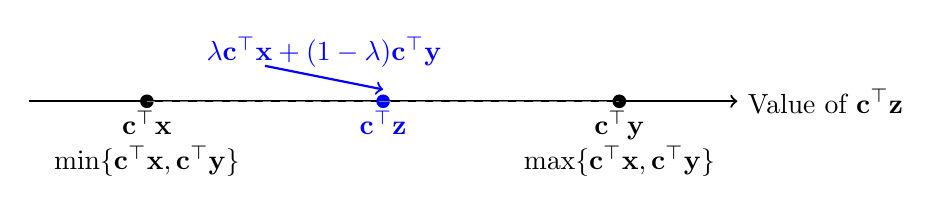
\begin{tikzpicture}[scale=1.5]
    % Draw the 1D line
    \draw[thick, ->] (0, 0) -- (6, 0) node[right] {Value of $\mathbf{c}^\top \mathbf{z}$};

    % Points for c^T x, c^T y, and c^T z
    \filldraw[black] (1, 0) circle (1.5pt) node[below] {$\mathbf{c}^\top \mathbf{x}$};
    \filldraw[black] (5, 0) circle (1.5pt) node[below] {$\mathbf{c}^\top \mathbf{y}$};
    
    % Point for c^T z (somewhere in between)
    \filldraw[blue] (3, 0) circle (1.5pt) node[below] {$\mathbf{c}^\top \mathbf{z}$};

    % Annotate convex combination
    \draw[dashed, gray] (1, 0) -- (3, 0);
    \draw[dashed, gray] (3, 0) -- (5, 0);

    % Add min and max bounds
    \node[below] at (1, -0.3) {$\min\{\mathbf{c}^\top \mathbf{x}, \mathbf{c}^\top \mathbf{y}\}$};
    \node[below] at (5, -0.3) {$\max\{\mathbf{c}^\top \mathbf{x}, \mathbf{c}^\top \mathbf{y}\}$};

    % Add explanation arrow for convex combination
    \draw[->, thick, blue] (2, 0.3) -- (3, 0.1) node[midway, above] {$\lambda \mathbf{c}^\top \mathbf{x} + (1-\lambda) \mathbf{c}^\top \mathbf{y}$};

\end{tikzpicture}
\end{center}



By the properties of convex combinations, the value \(\mathbf{c}^\top \mathbf{z}\) lies between \(\mathbf{c}^\top \mathbf{x}\) and \(\mathbf{c}^\top \mathbf{y}\). Formally:
\[
\min\{\mathbf{c}^\top \mathbf{x}, \mathbf{c}^\top \mathbf{y}\} \leq \mathbf{c}^\top \mathbf{z} \leq \max\{\mathbf{c}^\top \mathbf{x}, \mathbf{c}^\top \mathbf{y}\}.
\]



Therefore, the value of \(\mathbf{c}^\top \mathbf{z}\) is bounded above by \(\max\{\mathbf{c}^\top \mathbf{x}, \mathbf{c}^\top \mathbf{y}\}\), as required.
\end{proof}

\begin{theorem}{Optimal Solution at an Extreme Point}{}
\label{thm:extreme_point_optimum}
Let \(C \subseteq \mathbb{R}^n\) be a bounded, closed, and convex set. Let the objective be to maximize \(\mathbf{c}^\top \mathbf{x}\) over \(C\). Then, there exists an optimal solution \(\mathbf{x}^* \in C\) such that \(\mathbf{x}^*\) is an extreme point of \(C\).
\end{theorem}

\begin{proof}
Since \(C\) is bounded and closed, it is compact in \(\mathbb{R}^n\). The linear function \(\mathbf{c}^\top \mathbf{x}\) is continuous, and by the Extreme Value Theorem, it attains its maximum value on the compact set \(C\). Let \(\mathbf{x}^* \in C\) be such that:
\[
\mathbf{c}^\top \mathbf{x}^* = \max \{ \mathbf{c}^\top \mathbf{x} : {\mathbf{x} \in C} \}
\]

Suppose \(\mathbf{x}^*\) is not an extreme point of \(C\). Then, \(\mathbf{x}^*\) can be expressed as a convex combination of two distinct points \(\mathbf{x}, \mathbf{y} \in C\):
\[
\mathbf{x}^* = \lambda \mathbf{x} + (1-\lambda) \mathbf{y}, \quad \text{where } \lambda \in (0, 1).
\]

By Lemma~\ref{lemma:objective_bound}, the value \(\mathbf{c}^\top \mathbf{x}^*\) satisfies:
\[
\min\{\mathbf{c}^\top \mathbf{x}, \mathbf{c}^\top \mathbf{y}\} \leq \mathbf{c}^\top \mathbf{x}^* \leq \max\{\mathbf{c}^\top \mathbf{x}, \mathbf{c}^\top \mathbf{y}\}.
\]

Since \(\mathbf{x}^*\) maximizes \(\mathbf{c}^\top \mathbf{x}\) over \(C\), it must be that \(\mathbf{c}^\top \mathbf{x} = \mathbf{c}^\top \mathbf{x}^*\) and \(\mathbf{c}^\top \mathbf{y} = \mathbf{c}^\top \mathbf{x}^*\). Thus, both \(\mathbf{x}\) and \(\mathbf{y}\) also maximize \(\mathbf{c}^\top \mathbf{x}\) over \(C\).

If \(\mathbf{x}^*\) is not an extreme point, we can repeat this argument for \(\mathbf{x}\) and \(\mathbf{y}\), expressing them as convex combinations of other points in \(C\). However, since \(C\) is compact, this process must terminate after a finite number of steps, at which point we reach an extreme point that maximizes \(\mathbf{c}^\top \mathbf{x}\).

Hence, there exists an optimal solution at an extreme point of \(C\).
\end{proof}



\begin{theorem}{Extreme Points and Vertices of a Polyhedron}{}
Let \( P \subseteq \mathbb{R}^n \) be a polyhedron. Then, a point \( \mathbf{v} \in P \) is an extreme point if and only if \( \mathbf{v} \) is a vertex of \( P \).
\end{theorem}

\begin{proof}
\textbf{(If \( \mathbf{v} \) is not a vertex, then it is not an extreme point):}

Suppose \( \mathbf{v} \in P \) is not a vertex. By definition, this means \( \mathbf{v} \) is not the unique solution to any subset of \( n \) linearly independent constraints active at \( \mathbf{v} \). Let \( A' \mathbf{x} = \mathbf{b}' \) represent the active constraints at \( \mathbf{v} \), where \( A' \in \mathbb{R}^{m' \times n} \) (\( m' \leq n \)) is the matrix of active constraints, and assume the rows of \( A' \) are linearly independent. Since \( \mathbf{v} \) is not a vertex, the null space of \( A' \), denoted \( \mathcal{N}(A') \), is nontrivial, i.e., there exists a nonzero direction \( \mathbf{d} \in \mathbb{R}^n \) such that:
\[
A' \mathbf{d} = \mathbf{0}.
\]

Consider perturbing \( \mathbf{v} \) in the directions \( \mathbf{v} + \epsilon \mathbf{d} \) and \( \mathbf{v} - \epsilon \mathbf{d} \), for some small \( \epsilon > 0 \). Since \( \mathbf{d} \in \mathcal{N}(A') \), the perturbed points satisfy the active constraints:
\[
A' (\mathbf{v} + \epsilon \mathbf{d}) = A' \mathbf{v} + \epsilon A' \mathbf{d} = \mathbf{b}'.
\]
Similarly, \( A' (\mathbf{v} - \epsilon \mathbf{d}) = \mathbf{b}' \).

Furthermore, for sufficiently small \( \epsilon > 0 \), the perturbed points also satisfy all other constraints defining \( P \). This is because \( P \) is a polyhedron, and the constraints are continuous linear inequalities that remain satisfied under small perturbations of \( \mathbf{v} \).

Now, we express \( \mathbf{v} \) as a strict convex combination of \( \mathbf{v} + \epsilon \mathbf{d} \) and \( \mathbf{v} - \epsilon \mathbf{d} \):
\[
\mathbf{v} = \frac{1}{2} (\mathbf{v} + \epsilon \mathbf{d}) + \frac{1}{2} (\mathbf{v} - \epsilon \mathbf{d}).
\]
Since \( \mathbf{v} + \epsilon \mathbf{d} \neq \mathbf{v} \) and \( \mathbf{v} - \epsilon \mathbf{d} \neq \mathbf{v} \), and both points belong to \( P \), this shows that \( \mathbf{v} \) is not an extreme point of \( P \).


\begin{center}
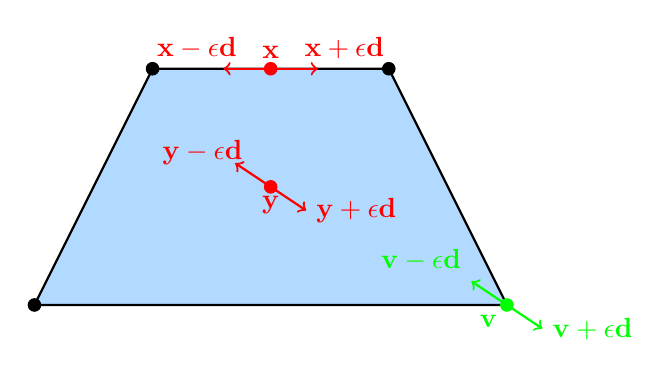
\begin{tikzpicture}[scale=1.5]
    % Draw the polytope
    \fill[blue!50!cyan,opacity=0.3] (0,0) -- (1,2) -- (3,2) -- (4,0) -- cycle;

    % Draw the edges of the polytope
    \draw[thick] (0,0) -- (1,2) -- (3,2) -- (4,0) -- cycle;

    % Label vertices
    \filldraw[black] (0,0) circle (1.5pt);
    \filldraw[black] (1,2) circle (1.5pt);
    \filldraw[black] (3,2) circle (1.5pt);
    \filldraw[green] (4,0) circle (1.5pt) node[below left] {$\mathbf{v}$};

    % Mark the point x on the edge
    \filldraw[red] (2,2) circle (1.5pt) node[above] {$\mathbf{x}$};

    % Draw the perturbation directions on the edge
    \draw[->, thick, red] (2,2) -- (2.4,2) node[midway, above right] {$\mathbf{x} + \epsilon \mathbf{d}$};
    \draw[->, thick, red] (2,2) -- (1.6,2) node[midway, above left] {$\mathbf{x} - \epsilon \mathbf{d}$};

    % Mark another point inside the polytope
    \filldraw[red] (2,1) circle (1.5pt) node[below] {$\mathbf{y}$};

    % Draw the perturbation directions inside the polytope
    \draw[->, thick, red] (2,1) -- (2.3,0.8) node[right] {$\mathbf{y} + \epsilon \mathbf{d}$};
    \draw[->, thick, red] (2,1) -- (1.7,1.2) node[midway, above left] {$\mathbf{y} - \epsilon \mathbf{d}$};

    % Draw perturbation directions for the green vertex
    \draw[->, thick, green] (4,0) -- (4.3,-0.2) node[right] {$\mathbf{v} + \epsilon \mathbf{d}$};
    \draw[->, thick, green] (4,0) -- (3.7,0.2) node[above left] {$\mathbf{v} - \epsilon \mathbf{d}$};

\end{tikzpicture}
\end{center}


\textbf{(If \(\mathbf{v}\) is a vertex, then it is an extreme point):}

Assume \( \mathbf{v} \in P \) is a vertex. By definition, there exists a subset of constraints, say \( A'\mathbf{x} = \mathbf{b}' \), where \( A' \in \mathbb{R}^{n \times n} \), such that \( \mathbf{v} \) is the unique solution to this system.

Suppose, for the sake of contradiction, that \( \mathbf{v} \) is not an extreme point. Then, \( \mathbf{v} \) can be expressed as:
\[
\mathbf{v} = \lambda \mathbf{x}_1 + (1 - \lambda) \mathbf{x}_2, \quad \mathbf{x}_1, \mathbf{x}_2 \in P, \, \lambda \in (0, 1),
\]
where \( \mathbf{x}_1 \neq \mathbf{v} \) and \( \mathbf{x}_2 \neq \mathbf{v} \).

We claim that both \( \mathbf{x}_1 \) and \( \mathbf{x}_2 \) must satisfy \( A'\mathbf{x} = \mathbf{b}' \).  To see this, 
let $\mathbf{a}$ be a row of $A'$ and $b$ be the corresponding right hand side value in $\mathbf{b}'$
By Lemma~\ref{thm:objective_bound}, the value of \( \mathbf{a}^\top \mathbf{z} \) satisfies:
\[
\min\{\mathbf{a}^\top\mathbf{x}_1, \mathbf{a}^\top\mathbf{x}_2\} \leq \mathbf{a}^\top\mathbf{v} \leq \max\{\mathbf{a}^\top\mathbf{x}_1, \mathbf{a}^\top\mathbf{x}_2\}.
\]
Since \( \mathbf{v} \) satisfies \( \mathbf{a}^\top\mathbf{v} = b\), this implies:
\[
\mathbf{a}^\top\mathbf{v} = \lambda \mathbf{a}^\top\mathbf{x}_1 + (1-\lambda) \mathbf{a}^\top\mathbf{x}_2 = b.
\]

If either \( \mathbf{a}^\top\mathbf{x}_1 \neq b \) or \( \mathbf{a}^\top\mathbf{x}_2 \neq b\), the equation above cannot hold. Hence, both \( \mathbf{x}_1 \) and \( \mathbf{x}_2 \) must satisfy \( \mathbf{a}^\top\mathbf{x} = b \).


Since \( \mathbf{v} \) satisfies \( A'\mathbf{x} = \mathbf{b}' \), both \( \mathbf{x}_1 \) and \( \mathbf{x}_2 \) must also satisfy \( A'\mathbf{x} = \mathbf{b}' \), as \( A'\mathbf{x} = \mathbf{b}' \) defines an affine subspace. However, this contradicts the assumption that \( \mathbf{v} \) is the unique solution to \( A'\mathbf{x} = \mathbf{b}' \).

Therefore, \( \mathbf{v} \) cannot be expressed as a strict convex combination of distinct points in \( P \), and \( \mathbf{v} \) is an extreme point.

\textbf{Conclusion:} A point \( \mathbf{v} \in P \) is an extreme point if and only if it is a vertex of \( P \).
\end{proof}



\subsection{Unbounded Sets and Rays}

\textbf{Rays and Directions:}  
A ray in \(\mathbb{R}^n\) is a set of points:
\[
\{\mathbf{x} : \mathbf{\bar x} + \lambda \mathbf{d}, \, \lambda \geq 0\},
\]
where \(\mathbf{\bar x}\) is the starting point and \(\mathbf{d}\) is the direction. Rays describe unbounded feasible regions in linear programming models.

\textbf{Extreme Directions:}  
An extreme direction is one that cannot be written as a positive combination of other directions. In linear programming, extreme directions help characterize unbounded solutions.

\medskip  
This section provides the mathematical tools essential for understanding and formulating linear programming problems, emphasizing the geometric and algebraic structures that define feasible regions and optimal solutions.

\begin{theorem}{Representation Theorem}{}
\label{thm:representation}
 Let  $\mathbf{x}^1, \mathbf{x}^2,\cdots \mathbf{x}^k$ be the set of extreme points of $P$, and if $P$ is unbounded, $\mathbf{d}^1, \mathbf{d}^2,\cdots \mathbf{d}^l$ be the set of extreme directions. Then any $\mathbf{x} \in P$ is equal to a convex combination of the extreme points and a non-negative linear combination of the extreme directions: $\mathbf{x} = \sum_{j=1}^k \lambda_j \mathbf{x}^j + \sum_{j=1}^l \mu_j \mathbf{d}^j$, where $\sum_{j=1}^k \lambda_j = 1$, $\lambda_j \ge 0,~\forall  j=1,2,\cdots,k$, and $\mu_j \ge 0,~\forall j=1,2,\cdots,l$.
 \end{theorem}

 \begin{minipage}[t][][b]{.4\linewidth}
\begin{align*}
\mbox{max~~} & z = -5x_1 - x_2  \\\
\mbox{s.t.~~} & x_1 - 4x_2 +s_1 = 0  \\
& -x_1 + x_2 + s_2 = 1 \\
& -x_1 + 2x_2 +s_3 = 4 \\
& x_1, x_2, s_1, s_2, s_3 \ge 0.
\end{align*}
\end{minipage}%
\begin{minipage}[t][][b]{.6\linewidth}
\begin{center}  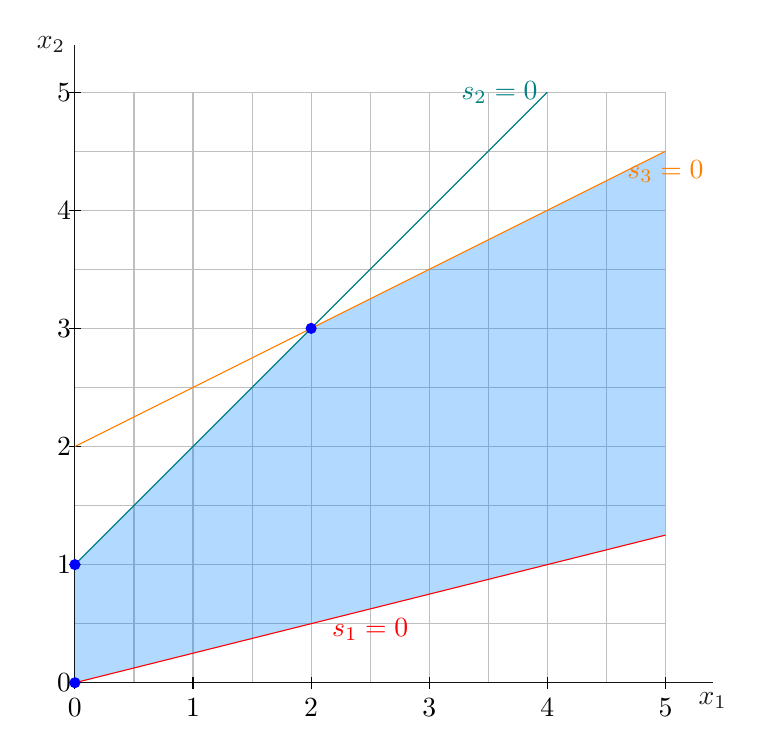
\begin{tikzpicture} [scale=1.5]
    \draw[gray!50, thin, step=.5] (0,0) grid (5,5);
    \draw[opacity=0.9] (0,0) -- (5.4,0) node[below] {$x_1$};
    \draw[opacity=0.9] (0,0) -- (0,5.4) node[left] {$x_2$}; % option \draw[very thick,->]

    \foreach \x in {0,...,5} \draw (\x,0.05) -- (\x,-0.05) node[below] {\x};
    \foreach \y in {0,...,5} \draw (-0.05,\y) -- (0.05,\y) node[left] {\y};

    \fill[blue!50!cyan,opacity=0.3] (0,0) -- (0,1) -- (2,3) -- (5,4.5) --(5,1.25)-- cycle;

    \draw [red](0,0) -- node[below] {$s_1=0$} (5, 1.25);
    \draw [teal] (0,1)  --  (4,5) node[left, sloped] {$s_2=0$};
    \draw [orange](0,2) --  (5,4.5) node[below, sloped] {$s_3=0$}; %node[above right ,sloped] 
    \node[fill=blue,circle,inner sep=0.05cm] at (0,0) {};
\node[fill=blue,circle,inner sep=0.05cm] at (0,1) {};
\node[fill=blue,circle,inner sep=0.05cm] at (2,3) {};

%	\filldraw[fill=red] (-0.05,-0.05) rectangle (0.05,0.05);
%	\filldraw[fill=red] (-0.05,.95) rectangle (0.05,1.05);
%	\filldraw[fill=red] (1.95,2.95) rectangle (2.05,3.05);
\end{tikzpicture} \end{center} 
\end{minipage}

Represent point (1/2, 1) as a convex combination of the extreme points of the above LP.  Find $\lambda$s to solve the following system of equations:

$$\lambda_1 \left[
  \begin{array}{c}
  0 \\
  0 \\
  \end{array} \right]+
 \lambda_2 \left[
  \begin{array}{c}
  0 \\
  1 \\
  \end{array} \right] +
 \lambda_3 \left[
  \begin{array}{c}
  2 \\
  3 \\
  \end{array} \right]  =
 \left[
  \begin{array}{c}
  1/2 \\
  1 \\
  \end{array} \right] 
$$

\section{Exercises}

\begin{ex}{Vector Operations}{}
Let \( \mathbf{v} = [3, -2, 4] \) and \( \mathbf{u} = [-1, 0, 2] \). Compute:
\begin{enumerate}
    \item \( \mathbf{v} + \mathbf{u} \)
    \item \( 2\mathbf{v} \)
    \item \( \mathbf{v} \cdot \mathbf{u} \)
\end{enumerate}
\end{ex}

\begin{ex}{Linear and Convex Combinations}{}
Let \( \mathbf{v}^1 = [1, 0] \), \( \mathbf{v}^2 = [0, 1] \), and \( \mathbf{v}^3 = [1, 1] \).

\begin{enumerate}
    \item Which of the following are linear combinations of \( \mathbf{v}^1 \) and \( \mathbf{v}^2 \)?  
    \begin{itemize}
        \item[(a)] \( [2, 3] \)  
        \item[(b)] \( [1, 1] \)  
        \item[(c)] \( [1, -1] \)
    \end{itemize}
    \item Is the vector \( [1/2, 1/2] \) a convex combination of any two of these vectors?
\end{enumerate}
\end{ex}
\begin{ex}{Linear Independence and Matrix Rank}{}
Consider the matrix \( A = \begin{bmatrix} 1 & 2 \\ 2 & 4 \end{bmatrix} \).
\begin{enumerate}
    \item Are the rows of \( A \) linearly independent?
    \item Are the columns linearly independent?
    \item What is \( \operatorname{rank}(A) \)?
\end{enumerate}
\end{ex}

\begin{ex}{Convex Combinations and Geometry}{}
Let \( P \) be the triangle with vertices at \( (0,0) \), \( (2,0) \), and \( (0,2) \).  
\begin{enumerate}
    \item Plot the set \( P \).
    \item Determine whether the point \( (1,1) \) is a convex combination of the vertices.
    \item Determine whether the point \( (1.5,1.5) \) is in \( P \).
\end{enumerate}
\end{ex}

\begin{ex}{Halfspace Geometry and Convexity}{}
Consider the halfspace \( H = \{ \mathbf{x} \in \mathbb{R}^2 : x_1 + 2x_2 \leq 4 \} \).
\begin{enumerate}
    \item Plot the halfspace and the boundary.
    \item Is the point \( (2,1) \) in \( H \)? What about \( (1,2) \)?
    \item Verify that the set is convex by checking whether the midpoint between \( (0,0) \) and \( (2,1) \) lies in \( H \).
\end{enumerate}
\end{ex}


